\subsection{GenI Honeynet}
Bei einem GenI Honeypot wird das gesamte Netz durch eine Firewall in drei Teile unterteilt. Der erste Teil ist das Produktivnetz indem sich das zentrale Management System befindet. Der zweite Teil ist das Internet, welcher das Zugangsmedium des Angreifers darstellt. Der dritte und letzte Teil ist das Honeynet. 

Der Prozess der Datensammlung beginnt bereits mit passieren der Firewall. Dort können Informationen wie die verwendeten Protokolle, Zeitstempel,IP-Adressen und Ports gesammelt werden. Außerdem wird hier kontrolliert wie oft der Angreifer eine Verbindung eingehen kann (Data Control). Wie viele Versuche zugelassen werden hängt vom Verwendungszweck des Honeynets ab. Der Router zwischen Honeynet und Firewall unterstützt diese auf zwei verschiedene weisen. Zum Einem versteckt er die Firewall vor dem Hacker. Der Angreifer denkt, er greift auf einen produktiven Router zu. Zum Anderen unterstützt er die Firewall in Sachen Zugriffskontrolle. So kann ein Single-Point-of-Failure vermieden werden. 

Ein IDS-System steht nun noch zwischen dem Angreifer und den Honeypots. Dieses ist meist über einen Switch (oder wie in Abb. \ref{hnet:geni} mit einem Router) mit dem gesamten Honeynet verbunden. Dort werden alle Netzwerkaktivitäten protokolliert und bei bestimmten Angriffsmustern gegebenenfalls ein Alarm ausgelöst. 
\\
\begin{figure}[ht]
    \centering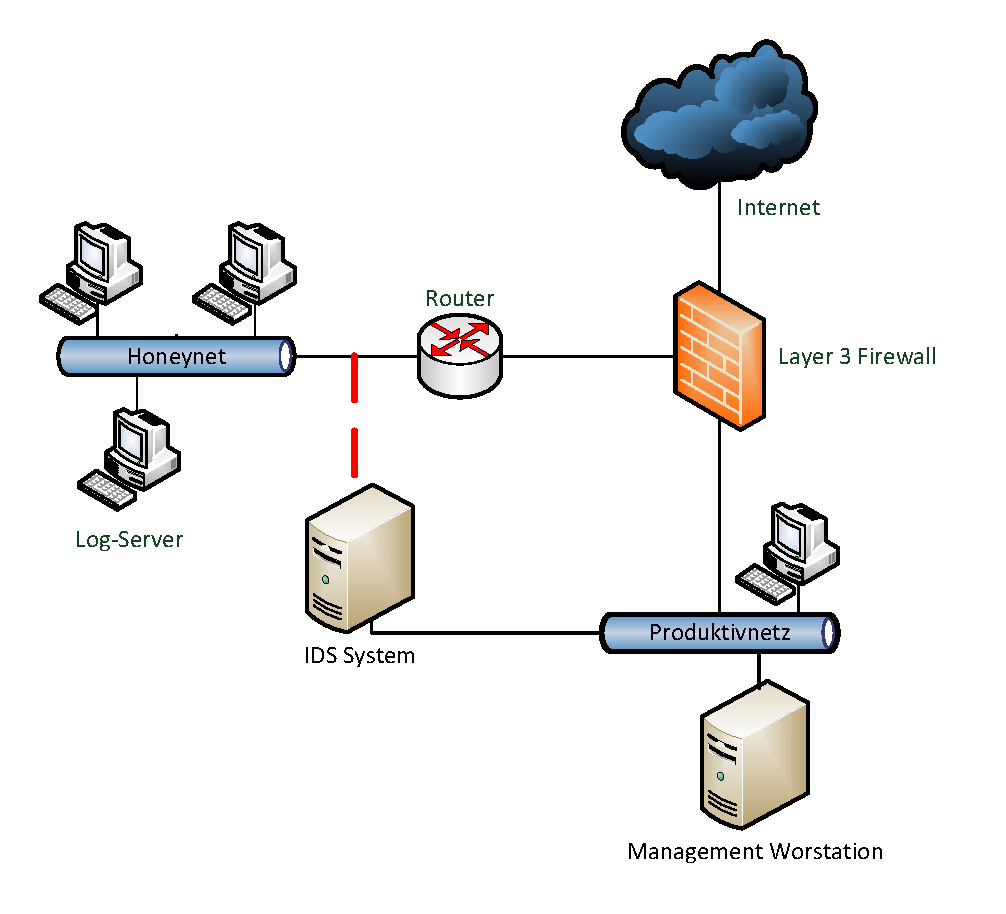
\includegraphics[scale=0.5]{Bilder/GenI.pdf}
  \caption{GenI Honeynet}
  \label{hnet:geni}
\end{figure}
\\